\documentclass[11pt]{aghdpl}
% \documentclass[en,11pt]{aghdpl}  % praca w języku angielskim

% Lista wszystkich języków stanowiących języki pozycji bibliograficznych użytych w pracy.
% (Zgodnie z zasadami tworzenia bibliografii każda pozycja powinna zostać utworzona zgodnie z zasadami języka, w którym dana publikacja została napisana.)
\usepackage[english,polish]{babel}


% Użyj polskiego łamania wyrazów (zamiast domyślnego angielskiego).
\usepackage{polski}

\usepackage[utf8]{inputenc}

% dodatkowe pakiety

\usepackage{mathtools}
\usepackage{amsfonts}
\usepackage{amsmath}
\usepackage{amsthm}

% --- < bibliografia > ---

\usepackage[
    backend=biber,
    style=authoryear-icomp,
    sortlocale=de_DE,
    natbib=true,
    url=false, 
    doi=true,
    eprint=false
]{biblatex}

\usepackage{csquotes}
% Ponieważ `csquotes` nie posiada polskiego stylu, można skorzystać z mocno zbliżonego stylu chorwackiego.
\DeclareQuoteAlias{croatian}{polish}

\addbibresource{bibliografia.bib}

% Nie wyświetlaj wybranych pól.
%\AtEveryBibitem{\clearfield{note}}


% ------------------------
% --- < listingi > ---

% Użyj czcionki kroju Courier.
\usepackage{courier}

\usepackage{listings}
\lstloadlanguages{TeX}

\lstset{
	literate={ą}{{\k{a}}}1
           {ć}{{\'c}}1
           {ę}{{\k{e}}}1
           {ó}{{\'o}}1
           {ń}{{\'n}}1
           {ł}{{\l{}}}1
           {ś}{{\'s}}1
           {ź}{{\'z}}1
           {ż}{{\.z}}1
           {Ą}{{\k{A}}}1
           {Ć}{{\'C}}1
           {Ę}{{\k{E}}}1
           {Ó}{{\'O}}1
           {Ń}{{\'N}}1
           {Ł}{{\L{}}}1
           {Ś}{{\'S}}1
           {Ź}{{\'Z}}1
           {Ż}{{\.Z}}1,
	basicstyle=\footnotesize\ttfamily,
}

% ------------------------

\AtBeginDocument{
	\renewcommand{\tablename}{Tabela}
	\renewcommand{\figurename}{Rys.}
}

% ------------------------
% --- < tabele > ---

\usepackage{array}
\usepackage{tabularx}
\usepackage{multirow}
\usepackage{booktabs}
\usepackage{makecell}
\usepackage[flushleft]{threeparttable}

% defines the X column to use m (\parbox[c]) instead of p (`parbox[t]`)
\newcolumntype{C}[1]{>{\hsize=#1\hsize\centering\arraybackslash}X}


%---------------------------------------------------------------------------

\author{Mateusz Wydmański, Michał Kałduś, Rafał Kwaśnik}
\shortauthor{M. Wydmański, M. Kałduś, R. Kwaśnik}

%\titlePL{Przygotowanie bardzo długiej i pasjonującej pracy dyplomowej w~systemie~\LaTeX}
%\titleEN{Preparation of a very long and fascinating bachelor or master thesis in \LaTeX}

\titlePL{Sprawozdanie z modelowania systemu ofiara-drapieżnik}
\titleEN{}


\shorttitlePL{Sprawozdanie z modelowania systemu ofiara-drapieżnik} % skrócona wersja tytułu jeśli jest bardzo długi
\shorttitleEN{}

\thesistype{}
%\thesistype{Master of Science Thesis}

\supervisor{dr inż. Jakub Porzycki}
%\supervisor{Marcin Szpyrka PhD, DSc}

\degreeprogramme{Informatyka}
%\degreeprogramme{Computer Science}

\date{2016}

\department{Katedra Informatyki Stosowanej}
%\department{Department of Applied Computer Science}

\faculty{Wydział Elektrotechniki, Automatyki,\protect\\[-1mm] Informatyki i Inżynierii Biomedycznej}
%\faculty{Faculty of Electrical Engineering, Automatics, Computer Science and Biomedical Engineering}

\acknowledgements{}


\setlength{\cftsecnumwidth}{10mm}

%---------------------------------------------------------------------------
\setcounter{secnumdepth}{4}
\brokenpenalty=10000\relax

\begin{document}
\nocite{*}
\titlepages

% Ponowne zdefiniowanie stylu `plain`, aby usunąć numer strony z pierwszej strony spisu treści i poszczególnych rozdziałów.
\fancypagestyle{plain}
{
	% Usuń nagłówek i stopkę
	\fancyhf{}
	% Usuń linie.
	\renewcommand{\headrulewidth}{0pt}
	\renewcommand{\footrulewidth}{0pt}
}

\setcounter{tocdepth}{2}
\tableofcontents
\clearpage

\chapter{Wprowadzenie}
\label{cha:wprowadzenie}

$$	\frac{dx}{dt} = \alpha x - \beta x y $$
$$	\frac{dy}{dt} = \delta xy - \gamma y $$

gdzie

\begin{eqwhere}[2cm]
	\item[$x$] liczebność populacji ofiary
	\item[$y$] liczebność populacji drapieżnika
	\item[$\frac{dx}{dt}$,$\frac{dy}{dt}$] przyrost populacji w jednostce czasu
	\item[$t$] czas
	\item[$\alpha$,$\beta$,$\delta$,$\gamma$] parametry opisujące interakcje między populacjami i właściwości populacji
\end{eqwhere}

\noindent Modele ofiar drapieżników są jednymi z najważniejszych elementów składających się na bio- i ekosystemy. Gatunki konkursują, ewoluują, rozprzestrzeniają się dla bolączki poszukiwania pożywienia i możliwości przedłużenia linii garunku. Konkurencja może przyjmować różne formy: drapieżnik-ofiara,wirus-system immulonogiczny, pasożyt-nosiciel, surowiec-konsument, itd. 

\noindent W 1926 słynny Włoski matematyk Vito Volterra zaproponował prosty model opisujący interakcje między ofiarą i drapieżnikiem. Bazuje na kilku założeniach dotyczących środowiska, w którym koegzystują populacje ofiar i drapieżników, to jest:

\begin{itemize}
	\item Ofiara ma zawsze wystarczająco dużo pożywienia.
	
	\item Zaopatrzenie w pożywienie drapieżników zależy wyłącznie od wielkości populacji ofiar.
	
	\item Tempo wzrostu populacji jest proporcjonalne do jej wielkości.
	
	\item Środowisko nie podlega zmianom na korzyść którejkolwiek z populacji, a ewolucja genetyczne jest niekonswekwentna.
	
	\item Drapieżniki mają ograniczony apetyt.
\end{itemize}

\noindent Równania Lotki-Volterry, to para równań różniczkowych I rzędu, nieliniowych.

\noindent Analiza równań mówi nam, że zmiana ilościowa populacji ofiar jest równa jej tempu wzrostu minus  tempo z jaką populacja drapieżników eliminuje ofiary ze środkowiska. Z drugiego zaś biegunu, tempo wzrostu populacji drapieżników jest równoważne tempu wzrostu zasilanym przez dostępność pożywienia minus tempo ubytku populacji na skutek śmierci naturalnej.

\noindent Portret fazowy modelu Lotki-Voleterry daje interesujące rezultaty.

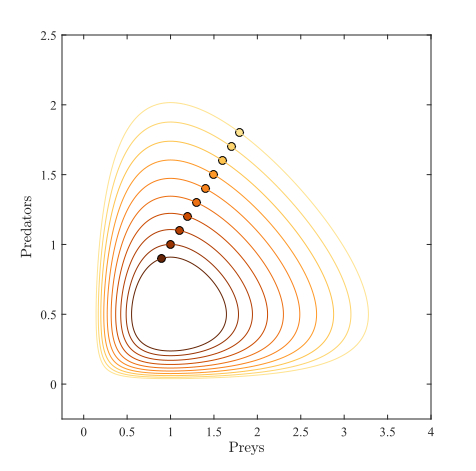
\includegraphics{img/symu}

\noindent Powyższy diagram pokazuje fluktuacje w ilości populacji ofiar i drapieżników. Koła zaznaczona na brzegach zamkniętych powierzchni pokazują warunki początkowe (dla stałych parametrów), gdzie ilości na osiach są rzędu $10^3$. W tym przypadku punktem stałym (populacje obu gatunków są ustalone i nie podlegają zmianom w czasie) jest punkt $(1;0.5)$. 

\noindent W modelu wyraźnie widać, że okres dobrego rozwoju drapiezników przypada gdy populacja ofiar jest duża. Jednakże, poprzez nadmierny rozrost i stopniowe malenie pokładów pożywienia, populacja drapieżników maleje. Wówczas, ofiary nie są na przysłowiowym „celowniku” i mają warunki do rozwoju. Koło się zatoczyło i cykl powtarza się.

\noindent Dla podanego systemu istnieją dwa ekwilibria. Jedno, punkt $(0;0)$, jest równoznaczne wymarciu obu populacji. Taki stan rzeczy będzie się miał  niezależnie od upływającego czasu. Podobnie, drugie ekwilibrium, z obiema populacjami o dodatnich wartościach, jest zależne od początkowych parametrow określających właściwości populacji ofiar i drapieznika.

\noindent Interesujące z biologicznego punktu widzenia jest stabilność układu dla drugiego ekwilibrium. 

\begin{equation}
\lambda_1=i\sqrt{\alpha\gamma} \quad \lambda_2=-i\sqrt{\alpha\gamma}
\end{equation}

\noindent Linearyzacja modelu wokół interesującego punktu: wartości własne jakobianu dla modelu przy drugim ekwilibrium są czysto urojone. Ten krytyczny punkt jest bifurkacją Hopfa – przy niewielkiej zmianie stabilność systemu zmienia się i pojawiają się rozwiązania okresowe. Warto podkreślić, że I metoda Lapunowa nie rozstrzyga o stabilności punktu równowagi, jeżeli system zlinearyzowany jest jedynie stabilny. \cite{Mit}

\noindent Punkt ustalony jest eliptyczny i na podstawie teorii Kolmongorova-Arnolda-Mosera (KAM), która daje odpowiedź na zachowanie w pobliżu punktów eliptycznych, populacje odchylone od punktu ustalonego będą podlegały oscylacjom z częstością $ \omega=\sqrt{\alpha\gamma} $.

\vspace{1cm}
\begin{figure}[ht]
	\centering
	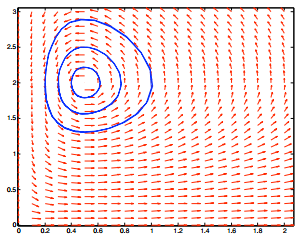
\includegraphics[width=0.6\textwidth]{img/phase}
	\caption{Portret fazowy przedstawionego modelu. Widać oscylujące wokół ekwilbrium rozwiązania i nieograniczony wzrost jednej populacji przy wymarciu drugiej}
\end{figure}














\chapter{Analiza modelu z zachowaniem stadnym}
\label{cha:spatial}

\section{Model matematyczny}

Model matematyczny opisujący zachowania ofiara-drapieżnik:

$$ \frac{\partial X}{\partial t} = rX(1-\frac{X}{K})-\frac{\alpha\sqrt{X}Y}{1+t_h \alpha\sqrt{X}}+d_x \bigtriangledown^2 X $$
$$ \frac{\partial Y}{\partial t} = sY^2+\frac{c\alpha\sqrt{X}Y}{1+t_h \alpha\sqrt{X}}+d_x \bigtriangledown^2 Y $$

gdzie 

\begin{eqwhere}[2cm]
	\item[$X$] liczebność populacji ofiary
	\item[$Y$] liczebność populacji drapieżnika
	\item[$r$] współczynnik przyrostu populacji ofiary
	\item[$K$] zdolność pojemnościowa układu
	\item[$\alpha$] efektywność poszukiwawcza populacji ofiar przez drapieżniki
	\item[$c$] współczynnik żarłoczności drapieżników
	\item[$t_h$] średni czas działania
	\item[$\frac{dx}{dt}$,$\frac{dy}{dt}$] współczynnik dyfuzji odpowiednich populacji
\end{eqwhere}

\noindent W powyższym modelu populacje poruszają się losowo - opisane poprzez model ruchów Browna. Zachowanie zostało uwzględnione w równaniach. Czas działania autor opracowania przyrównał do zera dla uproszczenia rozważań. $\bigtriangledown$ jest operatorem Laplace'a w przestrzeni dwuwymiarowej $R$ = ($R_1$,$R_2$) używanym dla wyrażenia ruchów populacji.

\section{Stabilność}

\noindent Interesuje nas stabilność tego systemu. Z biologicznego punktu widzenia jesteśmy zainteresowani w studiach zachowania koegzystujących populacji ofiar i drapieżnika. Niech punkt równowagi będzie postaci (x*,y*), gdzie obie populacje mają dodatnie wartości i żadna nie wymarła. Okazuje się, że takie ekwilibrium istnieje.

$$ x* = 1 - \frac{c}{s}, \quad y* = \frac{c}{s}\sqrt{x*}$$

\section{Bifurkacje}

\noindent Wraz ze zmianą niektórym parametrów (c,s) struktura jakościowa modelu może się dramatycznie zmienić. Bifurkacją nazywamy skokową zmianę właściwości modelu matematycznego przy niewielkiej zmianie parametrów. Przykładem może być liczba Reynoldsa, ważna w mechanice płynów bezwymiarowa liczba, która oszacowuje występujący podczas ruchu płynu stosunek sił bezwładności do sił lepkości. Przez zmianę tego parametru ruch płynu może zmienić się z laminarnego w falowy albo turbulentny.

\noindent W systemach reakcji-dyfuzji wyróżniamy dwa typy bifurkacji - Hopfa i Turinga. Interesującą bifurkacją jest ta druga, prowadzi bowiem do stanu, gdzie na całej modelowanej przestrzeni pojawiają wzory. W dwóch wymiarach są nimi zwykle heksagony lub figury o pasiastej aparycji.

\noindent W modelu możliwe jest wyznaczenie relacji między parametrem $s$ i $c$, dla którego wartość parametru $s$ będzie wartością krytyczną dla bifurkacji Hopfa i Turinga.

\begin{figure}[h]
	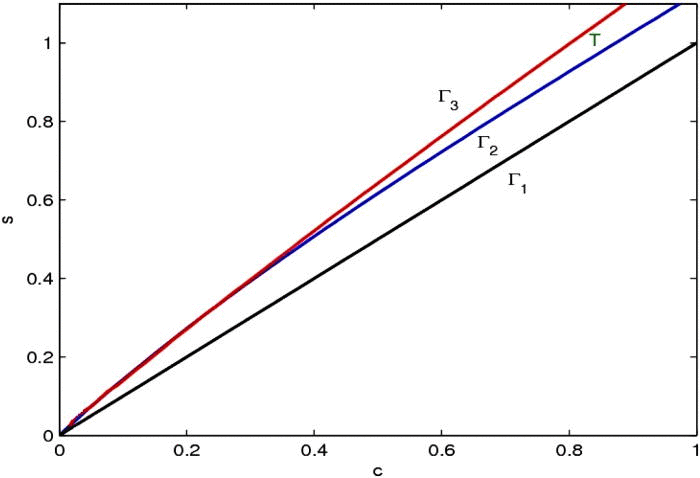
\includegraphics[width=\textwidth]{img/plane}
	\centering 
	\caption{Przestrzeń Turinga oznaczona jako T dla $\delta=10$. $\tau_1$,$\tau_2$,$\tau_3$ są kolejno są liniami bifurkacji Turinga, Hopfa, i ekwilibrium egzystencji.}
\end{figure}

\clearpage

\section{Symulacje}
\noindent Istotnie, interesujące zachowania ujawniają się dla wyznaczonych parametrów. Widoczne są różne kategorie wzorów na skutek bifurkacji Turinga dla różnych wartości parametrów w przestrzeni Turinga.


\begin{figure}[ht]
	\centering
	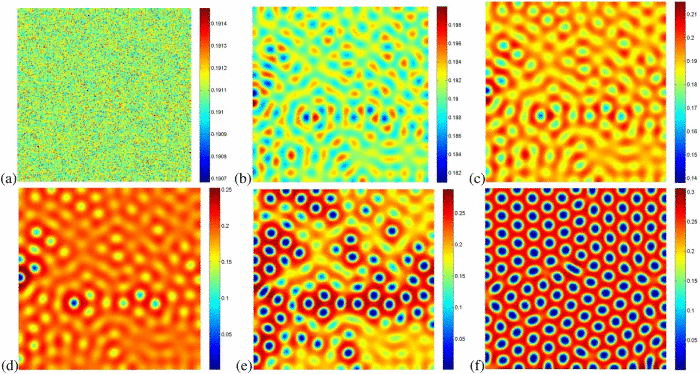
\includegraphics[width=0.6\textwidth]{img/3}
	
	\vspace*{\floatsep}% http://tex.stackexchange.com/q/26521/5764
	
	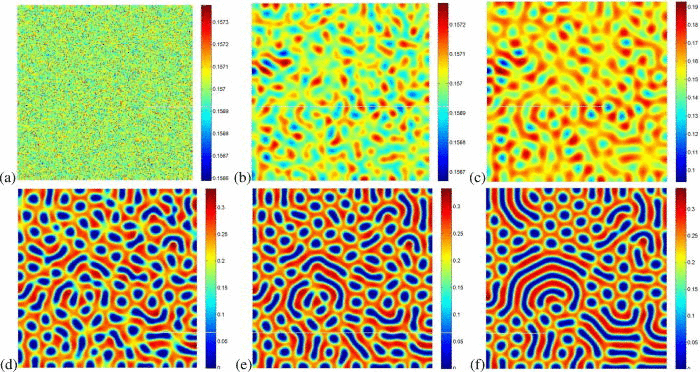
\includegraphics[width=0.6\textwidth]{img/2}
	
	\vspace*{\floatsep}% http://tex.stackexchange.com/q/26521/5764
	
	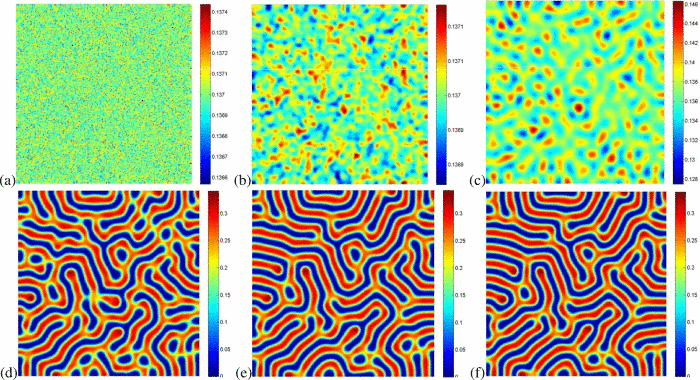
\includegraphics[width=0.6\textwidth]{img/1}
	
	\caption{Ewolucja zagęszczenia populacji ofiar w funkcji czasu}
\end{figure}


\chapter{Automaty komórkowe}

\section{Zagadnienie automatów}

\noindent Ciekawym zagadnieniem dotyczącym dzisiejszej informatyki jest symulacja  różnego rodzaju zjawisk, wydarzeń i populacji. Interesującą właściwością symulowanych modelów jest złożoność zachowań przy nakreśleniu prostych reguł działania. Na myśl nasuwa się pytanie: jakie zachowania będą przejawiały systemy zamodelowane bardziej wyrafinowanymi zasadami. Ograniczenia systemu w połączeniu z modelami matematycznymi oraz mocą obliczeniową komputerów mogą dać ciekawe rezultaty, których moglibyśmy nie przewidzieć. Utworzenie odpowiedniego modelu i wybranie odpowiednich warunków początkowych, pozwala nam też sprawdzić jak zachowa się dany system.
\noindent W celu zrealizowania podanego systemu jako program komputerowy na pomoc przychodzą nam automaty komórkowe. Dzięki prostocie zasad ich działania w bardzo krótkim czasie jesteśmy w stanie stworzyć prosty mechanizm, który będzie symulował rozwój populacji zwierząt. Stopniowo wprowadzając zasady działania populacji, od najprostszych jakimi jest poruszanie się i zdobywanie pokarmów, po te bardziej skompilowane jakimi jest rozmnażanie, uciekanie przed drapieżnikami czy polowanie na inne zwierzęta. Naszą uwagę przykuł fakt jak prosty jednowymiarowy automat komórkowy o prostych zasadach funkcjonowania może, przy niewiele różniących się od siebie regułach, dać zupełnie inny obraz wynikowy. Należy też zauważyć, że najwięcej funkcjonalności automatów komórkowych możemy znaleźć analizują właśnie jednowymiarowe  automaty. Tutaj definiujemy komórke oraz jej sąsiednie komórki, które znajdują się w pewnej odległości od niej. Dzięki temu jesteśmy za pomocą funkcji przejścia wyznaczyć następny stan danej komórki. 
\noindent Zaczniemy od tablicy jednowymiarowej i oznaczymy sobie dwa stany: 1 jako komórkę żywą, 0 jako komórkę  martwą, a jako sąsiadów przyjmiemy tylko te komórki,które znajdują się bezpośrednio przy niej. Ustalimy też, że następny stan będzie zależał bezpośrednio od stanu samej komórki oraz stanu sąsiadów. Wybierzemy też przejścia takie jak na tablicy.

\begin{table}[h!]
\centering
\begin{tabular}{ |c|c|c|c|c|c|c|c| } 
	\hline
	111 & 110 & 101 & 100 & 011 & 010 & 001 & 000\\
	0 & 0 & 1 & 0 & 0 & 1 & 1 & 0 \\
	\hline
\end{tabular}
\label{table:1}
\end{table}
\clearpage

\begin{figure}[ht]
	\centering
	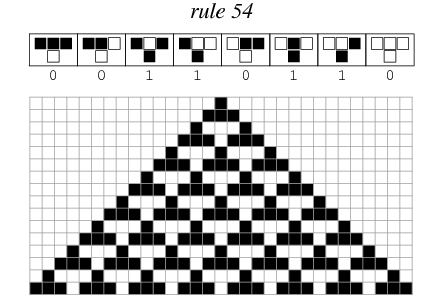
\includegraphics[width=0.8\textwidth]{img/triangle}
	\caption{rezultat wykonania operacji wedle tablicy powyżej}
\end{figure}

\section{Implementacja automatu}

\noindent Modelowanie populacji drapieżnik-ofiara za pomocą automatów komórkowych jest złożoną operacją. Każda komórka to zbiór stanów poszczególnych osobników. Każdy następny stan bazuje na poprzednim oraz na stanach sąsiadów.

\noindent Autorzy książki "A predator-prey model based on fully parallel cellular automata" przeprowadzi symulację na podstawie populacji wilków i owiec. Udało im się znaleźć trzy możliwe stany, do których będzie dochodził system. Są nimi:

\begin{itemize}
	\item współistnienie obu gatunków,
	\item rozwijanie się populacji ofiar,
	\item wyginięcie obu gatunków
\end{itemize}

\noindent Te stany zależały od ilości pożywania dla ofiar, czasu po jakim zwierzęta były wstanie się rozmnażać oraz sposobem opiekowania się na młodymi. Największym problemem z jakim spotkali się twórcy było to, że drapieżnik podczas polowania mógł zabić klika ofiar. Sposobem na poradzenia sobie  z tego typu zjawiskiem było wprowadzenie specjalnego sposobu doboru sąsiedztwa, które nie występowała w innych  automatach, a pozwala blokować możliwość zabicia wszystkich ofiar.  Dodatkowo dyskutowali też jaki wpływ na rozwoje populacji będą mieć takie czynniki jak zagęszczenie oraz mutacje poszczególnych gatunków. Zastanawiali się też jakie wtedy stany może osiągnąć taki automat.
\chapter{Równania Lotki-Volterry dla konkurencji}

\section{Model matematyczny}

\noindent Rozważając temat modelowania populacji za pomocą równań logistycznych warto poruszyć temat modelów uwzględniających również konkurencję o pożywienie i ogólnie system z wielogatunkowymi poziomami troficznymi.

\noindent W odpowiedzi przychodzi układ równań w formie podobnej do klasycznych, modelujących relacje ofiara-drapieżnik. Oparte są na bazie równań logistycznych postaci $\frac{d}{dx}f(x) = f(x)(1-f(x))$.  W przypadku standardowego układu Lotki-Volterry przypadkiem bazowym był wzrost wykładniczy.

\noindent Przypadek zająca i owcy mógłby zostać opisany następującym układem równań:

$$\frac{dN_1}{dt}=N_{1}r_{1}\left(1-\frac{\left({N_{1}+\alpha _{{12}}N_{2}}\right)}{K_1}\right)$$
$$\frac{dN_2}{dt}=N_{2}r_{2}\left(1-\frac{\left({N_{2}+\alpha _{{21}}N_{1}}\right)}{K_2}\right)$$

\begin{eqwhere}[2cm]
	\item[$r_1,r_2$] wzrost per capita członków poszczególnych populacji 
	\item[$\alpha_{nm}$] współczynnik konkurencji jednostki z populacji $m$ na jednostkę z populacji $n$
	\item[$K_1,K_2$] zdolność pojemnościowa układu dla poszczególnych populacji
\end{eqwhere}

\noindent Założeniem logistycznego modelu jest to, że liczba potomstwa per rodzic maleje liniowo ze wzrostem populacji tej populacji.

\noindent Włączając w to konkurencję innego gatunku, liczba potomstwa na rodzica zależy nie tylko od populacji pierwszej, ale również od populacji drugiej.

\newpage

\begin{figure}
	\centering
	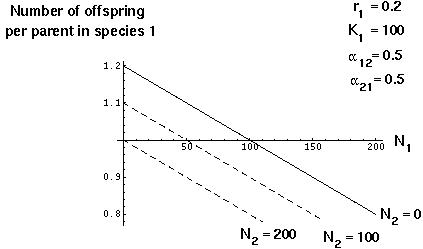
\includegraphics[width=\textwidth]{img/Fig1}
	\caption{Liczba potomków na dorosłego osobnika w funkcji parametrów}
\end{figure}

\section{Właściwości modelu}

\begin{itemize}[itemsep=0em]
	\item jeśli $\alpha_{12}$ wynosi zero, wtedy dynamika gatunku pierwszego będzie przedstawiona równaniem logistycznym (sigmoidalny wykres) 
	
	\item analagicznie dla $\alpha_{21} = 0$
	
	\item jeśli $\alpha_{12} < 0$ to populacja druga zwiększa liczbę surowców dostępnych dla populacji pierwszej
	
	\item jeśli oba współczynniki $\alpha_{12},\alpha_{21} = 0$ to relację między populacjami nazywamy mutualizmem
	
	\item jeśli $\alpha_{12}$ albo $\alpha_{21}$ jest równe zero (albo bardzo blisko zera), to mówimy że populacje są w relacji komensalizmu
	
	\item jeśli tylko jeden ze współczynników jest ujemny, a drugi dodatni, to mówimy, że populacje są w relacji pasożytnictwa
	
	\item jeśli oba współczynniki są dodatnie to populacje ze sobą konkurują
	
\end{itemize}

\section{Symulacje dla dodatnich współczynników}

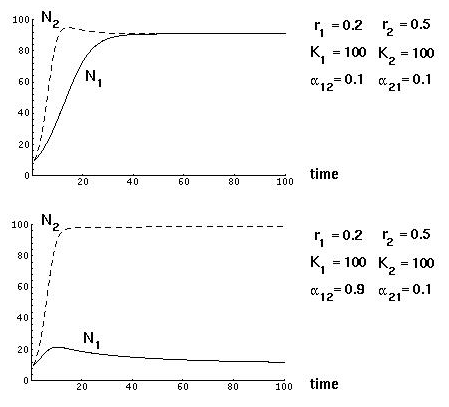
\includegraphics{img/Fig2}

\noindent Jeśli $\alpha_{12}$ i $\alpha_{21}$ są małe, to obie populacje osiągają ekwilibrium w pobliżu odpowiedniej pojemności systemu. Jeśli $\alpha_{12}$ jest znacznie większe od $\alpha_{21}$ (gatunek drugi ma większy impakt na liczebność gatunku pierwszego niż odwrotnie), wtedy liczebność gatunku pierwszego jest utrzymywana na niskim poziomie spowodowanym wyższością konkurencyjności drugiego gatunku.

\noindent Do stworzenia stabilnego ekosystemu wszyste wartości własne macierzy $a_{ij}$ muszą być dodatnie. Duże systemy Lotki-Volterry mogą osiągnąć stabilność jeśli współczynniki konkurencji $\alpha_{ij}$ mogą ewoluować zgodnie z naturalną selekcją (\cite{Kon} i \cite{Ack})




% itd.
% \appendix
% \include{dodatekA}
% \include{dodatekB}
% itd.

\printbibliography

\end{document}
